\documentclass[10pt]{article}
\usepackage[margin=0.85in]{geometry}
\usepackage{amsmath,amssymb,graphicx,booktabs,array,xcolor}
\usepackage[colorlinks=true,allcolors=blue]{hyperref}
\hypersetup{pdfauthor={Nima Kamali and Mert Turna},pdftitle={Scalar-Potential Action Experts: A Controlled LIBERO Study}}
\setlength{\parindent}{0pt}
\setlength{\parskip}{5pt}
\newcommand{\pihalf}{\pi_{0.5}}
\newcommand{\pending}{\textcolor{gray}{Pending}}
\title{Scalar-Potential Action Experts in a Pretrained\texorpdfstring{ $\pihalf$}{ pi0.5} Policy:\\A Controlled LIBERO Study}
\author{Nima Kamali and Mert Turna}
\date{22 November 2026}
\begin{document}
\maketitle
\begin{center}\small Evaluation snapshot of 22 November 2026, 14:43 UTC.\end{center}

\begin{abstract}
We study a conservative output parameterization for the action expert of a pretrained vision-language-action policy. The proposed expert forms one scalar potential from the dot product of its action input and its original vector output, and uses the full input gradient as its velocity. The experiment compares the potential expert with both a pretrained-output direct-field baseline and a zero-output direct-field control. All three arms retain the same frozen vision-language backbone, action-expert architecture, data, training exposure, and numerical protocol. The fixed evaluation comprises three paired training seeds, one and ten Euler steps, and 40 LIBERO tasks with 50 initial states per task; a released policy is evaluated separately, for 40,000 episodes in total. We compare matched ten-step rollouts of the potential expert and the reset direct-field control using the same training seed, task, and initial state. We report the paired success-rate comparison and identify the observations supporting it.
\end{abstract}

\section{Introduction}
Vision-language-action models combine pretrained visual and linguistic representations with an action-generating model. The $\pihalf$ system illustrates this approach at substantial scale \cite{pi05}. Here we ask a narrower question: does requiring an action expert's velocity to be the gradient of a scalar improve its behavior under a matched adaptation protocol? A conservative field is a structural constraint, not a guarantee of better optimization, better closed-loop control, or cheaper inference.

Our intervention preserves the pretrained host architecture and changes the interpretation of the complete action expert's output. The reset direct-field control separates this constraint from the effect of zero-output initialization. The experiment is a frozen-backbone adaptation study, not a reproduction of full vision-language-model fine-tuning. Its primary comparison is the potential model against the reset direct field at ten Euler steps. Comparisons to the pretrained-output baseline and results at one step are secondary.

\section{Related work}
Flow matching learns vector fields by regression along specified probability paths \cite{flowmatching}. We retain the host policy's interpolation, target, time distribution, and Euler sampler, rather than adopting a new transport objective. The reference model and released checkpoint come from the $\pihalf$/OpenPI family \cite{pi05,openpi}.

Scalar-energy parameterizations already appear in generative modeling and robotics. Sun et al. use an input--network-output dot product to define a flow potential, derive a time-dependent energy readout, and compose it with physical structure for PDE fields \cite{composing}. We reuse that parameterization within a pretrained action transformer. EnergyFlow instead replaces a conditional U-Net's vector output with temporal pooling and a scalar MLP head; it differentiates the scalar to obtain its field and studies reward recovery under additional assumptions \cite{energyflow}. Energy Matching uses a time-independent scalar formulation \cite{energymatching}, while Equilibrium Matching studies equilibrium rather than time-conditioned transport dynamics \cite{eqm}. Our contribution is the controlled pretrained-policy adaptation and its matched initialization experiment; neither scalar robot policies nor the dot-potential construction originate here. We do not test reward recovery, physical-energy composition, or equilibrium sampling.

LIBERO provides a robot-manipulation benchmark designed to study knowledge transfer \cite{libero}. We use the fixed four-suite, 40-task evaluation configuration stated below, not the benchmark's entire task collection. Work on Euler integration in flow policies motivates examining one-step and multi-step sampling on the same checkpoints \cite{onestep}; its empirical conclusions are not assumed to hold for our constrained expert.

\section{Method}
\subsection{Full-gradient dot potential}
Let $x\in\mathbb{R}^{H\times D}$ denote a noisy normalized action chunk, with $H=10$ and $D=32$, and let $c$ denote the cached image-language conditioning. The original action transformer produces $f_\theta(x,\tau,c)$ of the same shape. We define
\begin{align}
\Psi_\theta(x,\tau,c)&=\sum_{h=1}^{H}\sum_{d=1}^{D}x_{hd}f_{\theta,hd}(x,\tau,c),\\
v_\theta(x,\tau,c)&=\nabla_x\Psi_\theta(x,\tau,c)
=f_\theta(x,\tau,c)+J_{f_\theta}(x,\tau,c)^\top x.
\end{align}
The dot construction follows the potential parameterization of Sun et al.\ \cite{composing}, with the complete pretrained action expert replacing their field-generating backbone. The reduction is a sum, not a mean. The derivative includes every action-dependent layer and the output projection. Detaching the vector output would remove the Jacobian term and define a different model. A single scalar spans the complete chunk; coordinates and time steps are not assigned independent energies. The conditioning backbone is frozen, while the action expert and its input, output, and time projections are trainable.

The action expert retains width 1024, 18 transformer layers, and MLP width 4096. Its original smooth activations and adaptive normalization are retained. The policy uses the official LIBERO configuration with discrete state input disabled: the neural conditioning is images and language, although state remains part of observation processing. Only seven action coordinates are executed; the model and training objective retain all 32 channels. Conservativeness is defined in normalized action coordinates and should not be interpreted as invariance under arbitrary physical-unit rescaling.

The dot reduction introduces no additional learned parameters. Its fixed value at the origin is a potential gauge, not a restriction on the velocity at that point. In particular, for a differentiable potential $\phi$ on a star-shaped domain containing zero, define $g(x)=\int_0^1\nabla\phi(sx)\,ds$. The fundamental theorem of calculus gives $x^\top g(x)=\phi(x)-\phi(0)$. Thus the dot form can represent a potential up to an irrelevant additive constant when its vector function is unrestricted. This identity does not imply that the finite pretrained transformer realizes every such $g$, or that its optimization is equivalent to that of a scalar-output network.

The intervention changes computation despite preserving parameter count: each velocity requires a vector--Jacobian product, and training differentiates through that product. We therefore compare success at matched optimizer exposure and solver steps, while reporting computational cost separately. Equal parameter count or equal $K$ is not a claim of equal FLOPs, memory, or wall-clock time. Conservativeness holds for fixed conditioning and transport time; changing observations during closed-loop control does not define a single global Lyapunov function.

\begin{figure}[t]
\centering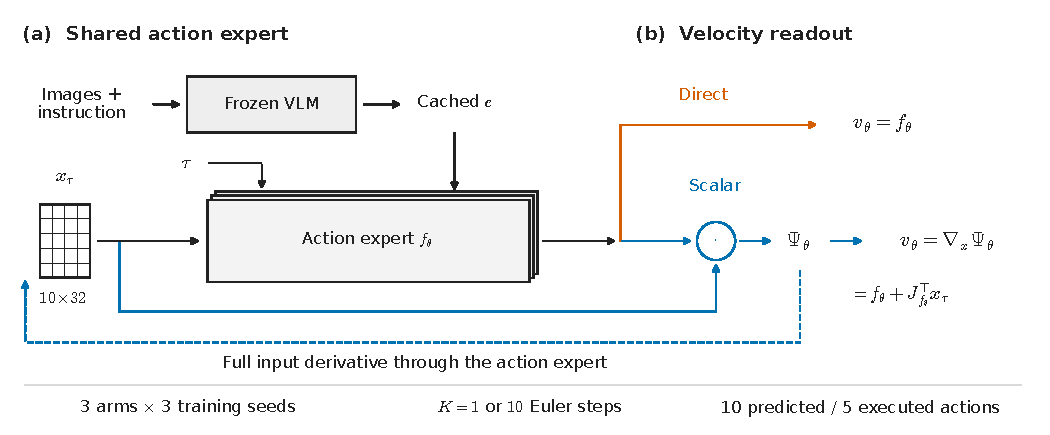
\includegraphics[width=\linewidth]{figures/method.pdf}
\caption{The scalar intervention reuses the complete action expert. The input-gradient path is retained through the vector output; the frozen conditioning cache is shared across solver steps. This is an architecture diagram, not a measured performance result.}
\label{fig:method}
\end{figure}

\subsection{Objective and inference}
For a normalized demonstration chunk $A$ and independent Gaussian noise $\epsilon$, the training path and target are
\begin{equation}
x_\tau=(1-\tau)A+\tau\epsilon,\qquad u=\epsilon-A,\qquad
\epsilon\sim\mathcal{N}(0,I),\quad \tau=0.001+0.999\,\mathrm{Beta}(1.5,1).
\end{equation}
All arms minimize the same mean squared velocity error over the complete action tensor. Training the potential model differentiates the input gradient with respect to its parameters; the required higher-order gradient is part of the computation. Inference starts at $\tau=1$ and uses $K\in\{1,10\}$ negative Euler increments to reach zero, with the same terminal checkpoints and paired noise schedule. An input-gradient velocity evaluation is not cost-equivalent to a direct-field evaluation, even when the number of solver steps is equal.

For this interpolation, the associated scalar energy readout can be written, up to a context/time offset, as
\begin{equation}
E_\theta(x,\tau,c)=\frac{\lVert x\rVert^2+2(1-\tau)\Psi_\theta(x,\tau,c)}{2\tau}+b(\tau,c).
\end{equation}
This expression is singular at zero and does not by itself establish a calibrated reward or cross-context confidence score. The time-conditioned sampler is not an autonomous energy-descent procedure. No energy-based early stopping or extra refinement is introduced.

\section{Experimental setup}
\subsection{Controls and training}
\begin{table}[t]
\centering
\begin{tabular}{llll}
\toprule Arm & Trunk & Output initialization & Velocity \\
\midrule B0 & Pretrained & Pretrained & $f_\theta$ \\
B1 & Same pretrained trunk & Zero weight and bias & $f_\theta$ \\
P & Same initial tensors as B1 & Zero weight and bias & $\nabla_x(x^\top f_\theta)$ \\
\bottomrule
\end{tabular}
\caption{Matched controls. Each research arm uses seeds 17, 42, and 93, 30,000 updates, and the same frozen-backbone numerical protocol.}
\label{tab:design}
\end{table}

B1 and P begin with identical tensors and zero velocity. The zero projection permits its own parameters to learn immediately; a zero action-trunk gradient on the first update is expected. B0 retains the pretrained output. These controls isolate initialization from output parameterization without replacing the pretrained expert or freezing it to a small head.

We completed nine training runs using the full official LIBERO training set and the base checkpoint: B0, B1, and P at seeds 17, 42, and 93. Each run completed 30,000 optimizer updates with effective batch 256, using gradient accumulation to preserve that batch size. AdamW uses $(\beta_1,\beta_2)=(0.9,0.95)$, $\epsilon=10^{-8}$, weight decay $10^{-10}$, and global gradient clipping at 1.0. The learning rate warms up linearly for 10,000 updates to $5\times10^{-5}$ and remains at that value. EMA decay is 0.999; the predeclared terminal EMA checkpoint is evaluated. Terminal checkpoint hashes establish completed training.

All research arms use the same hybrid precision protocol: the frozen vision-language backbone is BF16 except its declared FP32 embedding/normalization parameters, and the trainable action expert, optimizer, and EMA remain FP32. Execution is eager with \texttt{highest} FP32 matmul precision. Native mixed checkpoint dtypes and exact recovery checks are retained. Earlier rejected or diagnostic precision protocols are not pooled into this study.

\subsection{Fixed evaluation grid}
The evaluation uses \texttt{libero\_spatial}, \texttt{libero\_object}, \texttt{libero\_goal}, and \texttt{libero\_10}, with ten tasks per suite and 50 official initial states per task. Each checkpoint/K pair therefore contains 2,000 episodes. Three arms, three seeds, and two K values yield 36,000 research episodes. The released LIBERO checkpoint is evaluated at both K values as a separate reference, adding 4,000 episodes. The complete result has 20 checkpoint/K batches and 80 checkpoint/K/suite cells.

The rollout and paired-noise seeds are both 7. Per-query noise identities are deterministic functions of task, initial state, and query index, shared across methods and K. Action horizon 10, replanning horizon 5, settling, camera orientation, transformations, and suite-specific limits follow the frozen runner. Policy-caused invalid actions count as failures; infrastructure interruptions retain separate attempts and do not silently contribute partial or duplicate trials. All evaluated task identities occur in the training data; these results must not be described as unseen-task generalization.

\subsection{Execution and numerical qualification}
Each checkpoint, solver-step, task and initial-state identity contributes exactly once. Infrastructure failures are retained separately, and the successful replacement attempts are selected explicitly without changing the original scientific settings.

Task processes retain the physical GPU, driver, container, and serving-runtime identity for each episode.\footnote{Evaluation began on NVIDIA H100 PCIe GPUs and expanded to include A100 GPUs. In the retained fixed-input captures, 33,120 of 33,600 A100 PCIe scalar action comparisons across two repeats exceeded the componentwise tolerance $10^{-5}+1.3\times10^{-6}|a_{\rm H100}|$. A100 PCIe therefore did not pass the unchanged H100 numerical gate; its tolerance was not widened. A100 SXM4 rollouts also lack accepted cross-H100 qualification in the retained evidence. These rollouts contribute only to descriptive observed-support results. Timing remains stratified by hardware.}

Some tasks execute concurrently on one GPU with independent policy/simulator processes and random-number states. Paired A100 tasks use disjoint CPU affinity partitions. Every task retains its original 50 episodes and scientific configuration. We stratify timing by hardware, runtime, model, solver steps, task, and concurrency, including recorded changes in concurrent workloads. Aggregate throughput counts unique completed episodes over a common wall-clock window; it is not calculated by summing reciprocal episode durations. Comparisons across different task mixes remain descriptive. Runtime records link each task to its hardware and concurrent workload.

\section{Analysis and results}
The registered full-study analysis requires the entire matrix and rejects missing, duplicated, mismatched, or partial records while checking checkpoint, protocol, seed, solver, and provenance identities. The descriptive observed-support analysis instead uses the retained, explicitly selected task outcomes and reports original phase validation separately. The primary endpoint is P minus B1 at K=10. P minus B0, the K=1 architecture comparisons, and within-model K=1 versus K=10 comparisons are secondary. Released-policy results remain separate from independent training-seed replicates.

Uncertainty uses 10,000 paired percentile-bootstrap resamples with analysis seed 0. The same training seeds are resampled on both sides; within each fixed task, initial-state draws are shared across the sampled seeds and compared methods. Tasks and suites receive equal weight. The 95\% intervals describe training-seed and initial-state variability on this fixed benchmark, with only three training seeds. They do not establish equivalence when a contrast is nonsignificant, nor support generalization to an unobserved task distribution. Secondary contrasts are reported as such, without inventing a multiplicity-adjusted decision rule after seeing outcomes.

For the current snapshot we apply the paired success-rate contrast to available common support. We match training seed, task, initial state, noise and execution settings within each pair. We average within each observed seed and task, then equally across represented seeds within each task, tasks within each suite, and suites. The analysis combines 1,150 on NVIDIA A100-PCIE-40GB and 750 on NVIDIA A100-SXM4-40GB and 4,100 on NVIDIA H100 PCIe. These observations cover 120 of the 120 planned seed--task combinations. All 6,000 planned primary pairs are present. The point estimate reproduces the registered complete-grid estimator. The descriptive interval below reuses the original bootstrap; a hardware-qualified confirmatory interval is not asserted.


\begin{table}[!htbp]\centering\small
\begin{tabular}{lrrrr}\toprule
& \multicolumn{2}{c}{$K=1$} & \multicolumn{2}{c}{$K=10$} \\
\cmidrule(lr){2-3}\cmidrule(lr){4-5}
Checkpoint & Successes & Archived & Successes & Archived \\ \midrule
B0, seed 17 & 1,841 & 0 & 1,822 & 0 \\
B0, seed 42 & 1,859 & 2,000 & 1,793 & 2,000 \\
B0, seed 93 & 1,847 & 0 & 1,820 & 0 \\
\addlinespace[3pt]
B1, seed 17 & 1,879 & 0 & 1,841 & 0 \\
B1, seed 42 & 1,856 & 2,000 & 1,809 & 2,000 \\
B1, seed 93 & 1,859 & 0 & 1,815 & 0 \\
\addlinespace[3pt]
P, seed 17 & 1,861 & 2,000 & 1,822 & 2,000 \\
P, seed 42 & 1,865 & 2,000 & 1,827 & 2,000 \\
P, seed 93 & 1,892 & 0 & 1,834 & 0 \\
\addlinespace[3pt]
Released reference & 1,932 & 0 & 1,917 & 0 \\
\bottomrule\end{tabular}\caption{Complete outcome counts. Each solver setting contains 2,000 selected episodes per checkpoint. Archived counts refer to the original accepted phase archives (16,000 episodes overall), not to the 40,000 selected rows that passed task-level validation. The cross-device qualification limitation applies to all mixed-device comparisons.}\label{tab:observed}\end{table}


\subsection{Descriptive complete-grid contrasts}
The final retained grid contains 40,000 non-infrastructure episodes. All 800 selected task logs pass the unchanged original row validator and have closed execution evidence. Four initial infrastructure-failure records remain in the audit package; only their explicitly recorded retries enter these statistics. Row and lifecycle validation is distinct from cross-device numerical qualification.
\begin{table}[htbp]\centering\small
\begin{tabular}{llrrr}\toprule
Contrast & Endpoint & Pairs & Difference & 95\% interval \\ \midrule
P $K=10$ minus B1 $K=10$ & Primary & 6,000 & +0.30 & [-1.27, +1.75] \\
P $K=1$ minus B1 $K=1$ & Secondary & 6,000 & +0.40 & [-1.18, +2.00] \\
P $K=1$ minus B0 $K=1$ & Secondary & 6,000 & +1.18 & [-0.20, +2.55] \\
P $K=10$ minus B0 $K=10$ & Secondary & 6,000 & +0.80 & [-0.58, +2.25] \\
B0 $K=1$ minus B0 $K=10$ & Secondary & 6,000 & +1.87 & [+0.27, +3.48] \\
B1 $K=1$ minus B1 $K=10$ & Secondary & 6,000 & +2.15 & [+1.05, +3.23] \\
P $K=1$ minus P $K=10$ & Secondary & 6,000 & +2.25 & [+1.05, +3.43] \\
Released $K=1$ minus Released $K=10$ & Secondary & 2,000 & +0.75 & [-0.15, +1.70] \\
\bottomrule\end{tabular}
\caption{Descriptive paired success-rate differences on the complete observed grid, in percentage points. The original paired-bootstrap calculation uses 10,000 resamples and random seed 0. Secondary intervals are not adjusted for multiple comparisons. The released policy has one checkpoint, so its interval describes paired initial-state variation rather than training-seed replication. Unresolved hardware eligibility prevents interpreting these intervals as the registered confirmatory analysis.}
\label{tab:descriptive-contrasts}\end{table}
% Descriptive report SHA256: a99687a59715cba9fe7ed2ffeab9a6825896e3719a57967e34d7b39eb9a6db9c


The descriptive 95\% interval for this difference was [-1.27, +1.75] percentage points. These mixed-hardware observations do not establish a confirmatory benefit under the registered numerical-eligibility criteria.

\section{Limitations and reporting}
The scalar constraint may aid or hinder optimization, and its higher-order computation can increase latency. A mathematically conservative field does not imply improved robot success. The study uses a frozen pretrained backbone and tasks represented in its training data, limiting claims about full-model adaptation and new-task transfer. Three training seeds provide a limited estimate of training variability. The retained A100 PCIe fixed-input capture failed the predeclared H100 numerical gate, and A100 SXM4 rollouts lack accepted cross-H100 qualification. Statistics combining these producers describe observed outcomes and do not establish the predeclared confirmatory comparison. Matching task placement by hardware where possible reduces, but does not eliminate, this concern. Complete row and lifecycle validation does not substitute for numerical qualification. Timing measurements remain stratified by hardware.

The final selected grid is complete: every checkpoint, solver-step, task and initial-state identity is present exactly once. The 16,000 episodes marked as phase validated refer to the original accepted phase archives; all 40,000 selected rows have separate task-validation and closed-lifecycle evidence. The distinction is retained rather than upgrading hardware eligibility from successful execution.

\section{Reproducibility}
The study's frozen worker commit is \texttt{a9c0bdbf5f20356246f25ec303c51e466fa4c3a3}; the full manifest SHA-256 begins \texttt{9e2036f5f8a78258}. The reproducibility index records full hashes for the manifest, methods and configuration sources, analysis entrypoint, and finalization interfaces. The retained evidence distinguishes original accepted phase archives, task-level row and lifecycle validation, and hardware qualification. No fully accepted 40,000-episode archive is asserted while hardware eligibility remains unresolved.

The portable dataset contains the 40,000 selected episodes in CSV and JSONL, 800 curated task records with source digests and scientific provenance, the effective attempt selections, checksums, and four excluded infrastructure records. Private identifiers and paths are omitted; original evidence is unchanged. The editable source package includes the original pinned statistical functions and a portable descriptive-analysis entrypoint. The eight contrasts reuse the original estimator on the complete observed grid without asserting hardware qualification.

\section{Conclusion}
On matched ten-step LIBERO rollouts, the scalar-potential expert had a success rate 0.30 percentage points higher than the reset direct-field control. The descriptive 95\% interval was [-1.27, +1.75] percentage points; unresolved hardware eligibility prevents a confirmatory benefit claim.



\begingroup\footnotesize\setlength{\parskip}{0pt}
\enlargethispage{2\baselineskip}
\bibliographystyle{plain}
\bibliography{references}
\endgroup
\end{document}
